\section{Detector calibration and commissioning}

\subsection{Pre-beam calibration}
Initial checkout and calibrations of the FT detectors upon completion of the installation were performed via:
\begin{itemize}
    \item Pulser, LED and cosmic ray runs for the FT-Cal;
    \item Pulser and cosmic ray runs for the FT-Hodo;
    \item Pulser and pedestal runs for the FT-Trk.
\end{itemize}

\subsubsection{FT-Cal pre-beam calibration}
Initial checkout of the calorimeter is performed via pulser and LED runs. 

In pulser runs, an external clock is used to trigger the readout of the entire FT-Cal recording the full fADC waveforms in a 400 ns window in the absence of a physics signal to measure baselines and monitor noise, for the purpose of identifying disconnected or malfunctioning channels. For each crystal, several parameters such as the average pedestal, the event-by-event pedestal RMS or the noise defined as the sample-by-sample pedestal RMS. The analysis can be performed online, connecting to the DAQ Event Transfer (ET) ring \cite{daq}, or from a recorded EVIO file using the FT Java calibration suite \cite{reconstruction}. Figure \ref{fig:ftcal_pulserrun} shows a view of a typical pulser run analysis as displayed by the calibration suite. Among the most useful information available from this analysis is the channel average noise that is indicative of its functionality: a noise level below the typical range is indicative of a malfunctioning preamplifier or disconnected cable while a noise level above the the typical range can indicate a high-voltage issue since the noise introduced by the LAAPDs is higher when the biased voltage is not applied. 

\begin{figure}
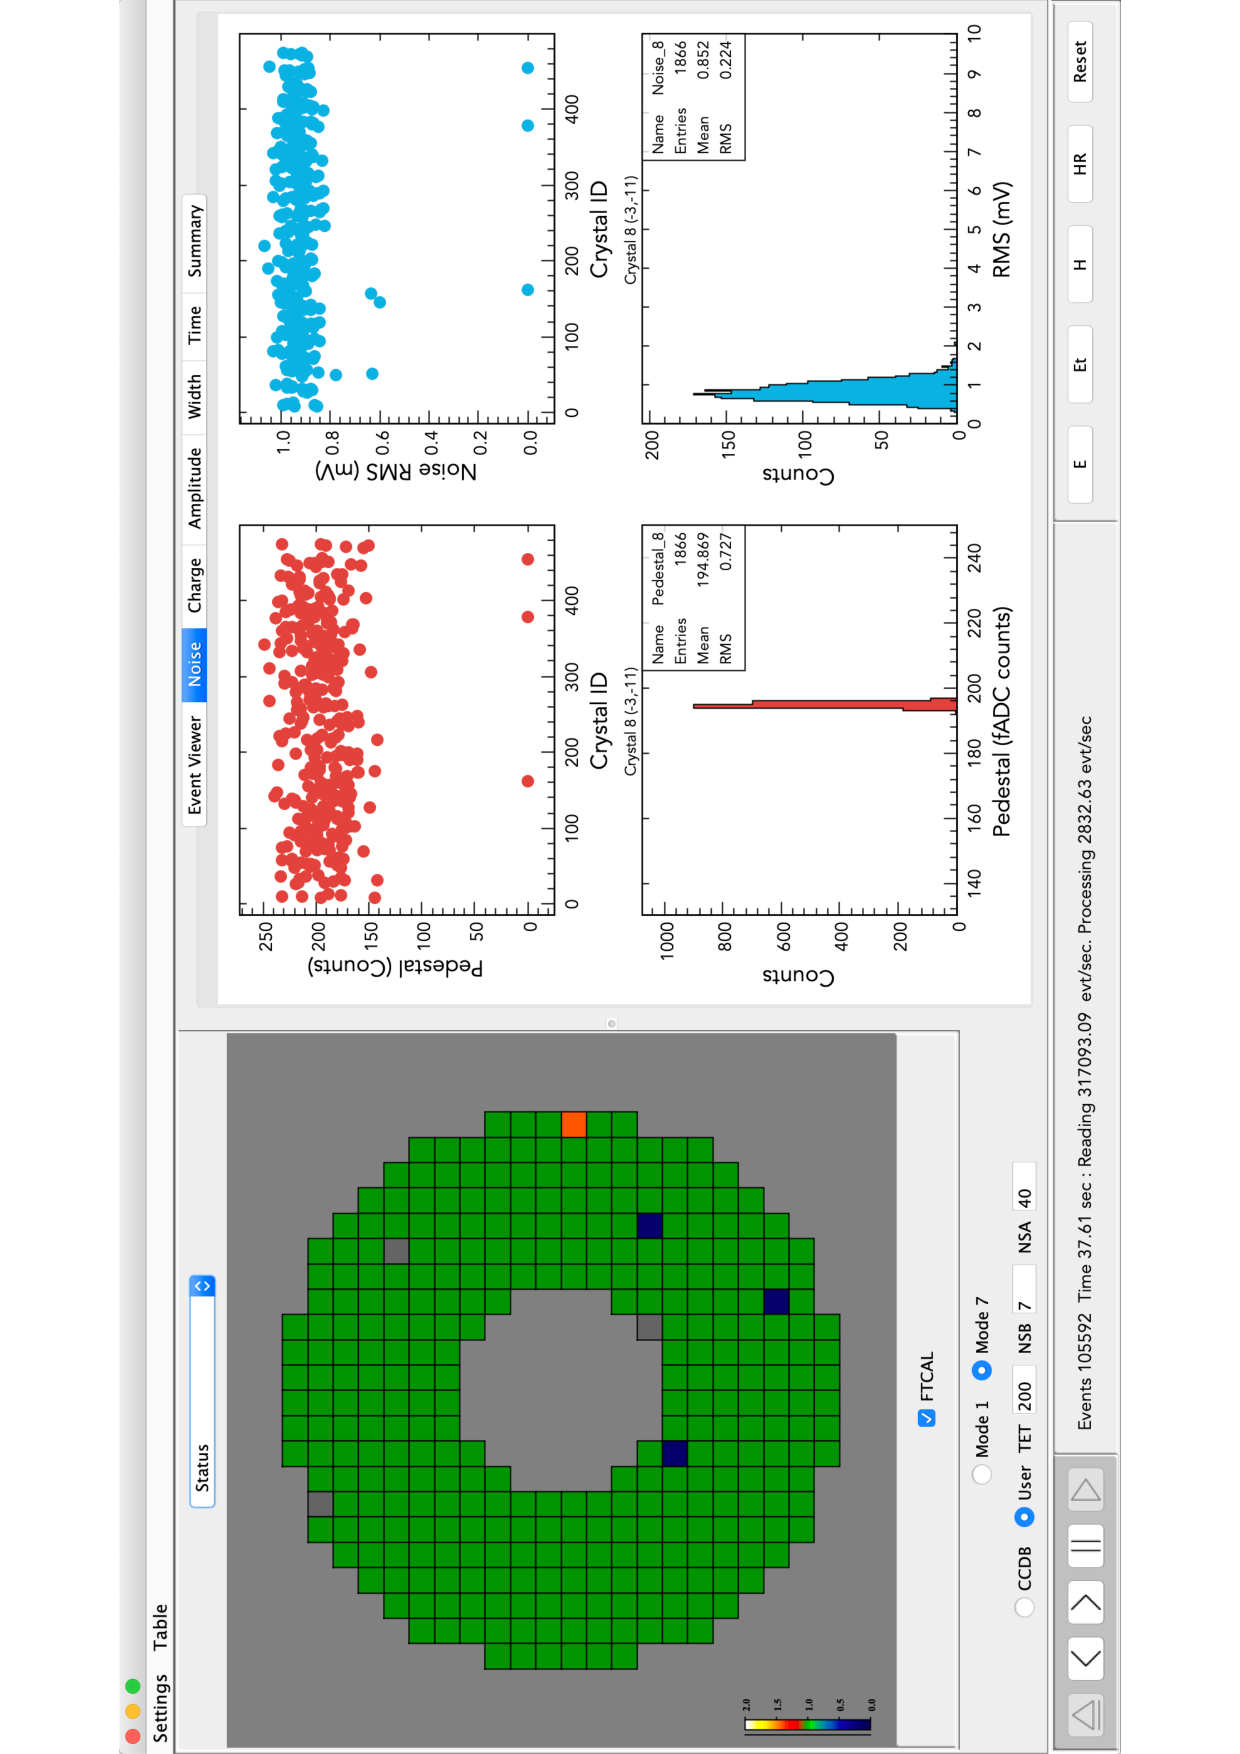
\includegraphics[height=1.0\columnwidth,angle=270]{fig/ftcal_pulserrun.pdf}
\caption{Results of the FTCal noise analysis from a pulser run. The left part of the calibration suite display shows a view of the calorimeter with a color scheme representing the status of the crystal: green corresponds to a fully functional element, blue to an elements with noise below the typical range that is indicative of a low gain preamplifier, orange to an element with noise above the typical range and gray to a crystal for which no data were recorded. The right part of the panel shows the average pedestal and noise as a function of the crystal number, and the event distribution of the pedestal and noise for the selected crystal.}
\label{fig:ftcal_pulserrun}
\end{figure}

Once the initial debugging of the system is completed based on pulser runs, a second checkout is performed based on LED runs. In this case, the FT-Cal LMS is used to input light in each of the calorimeter crystals and the corresponding signals are recorded to check the pulse amplitude and shape and assess the correct functioning of the LAAPDs, preamplifiers and front-end electronics. Using the EPICS slow controls interface of the LMS, the LEDs are switched on in groups of 6, one per driver, in a predefined sequence and pulsed at a rate of 62.5 Hz for a time interval of 30 s to accumulate about 1800 waveforms per channel. The LED pulse amplitudes have been tuned to provide a maximum amplitude at the fADC of about 1 V, which is representative of a typical signal expected for the calorimeter. The recorded waveforms are analyzed to extract the pulse amplitude as a function of time. In fact, upon being turned on, the LED light intensity undergoes an exponential drop until it reaches stability. This happens typically within 6-8 s. The amplitude in the stability region is fitted to a constant to extract the average value that is recorded and compared to reference values to detect changes in the detector response and potential failures. Fig. \ref{fig:ftcal_ledrun} shows the results of the analysis of a typical LED run as displayed by the calibration GUI. In the specific case, the analysis shows a relatively uniform response to the LED light, with typical amplitudes of the order of 1 V as defined by design, with few problematic channels that coincides with the ones identified by the pulse runs of Fig. \ref{fig:ftcal_pulserrun}. 


\begin{figure}
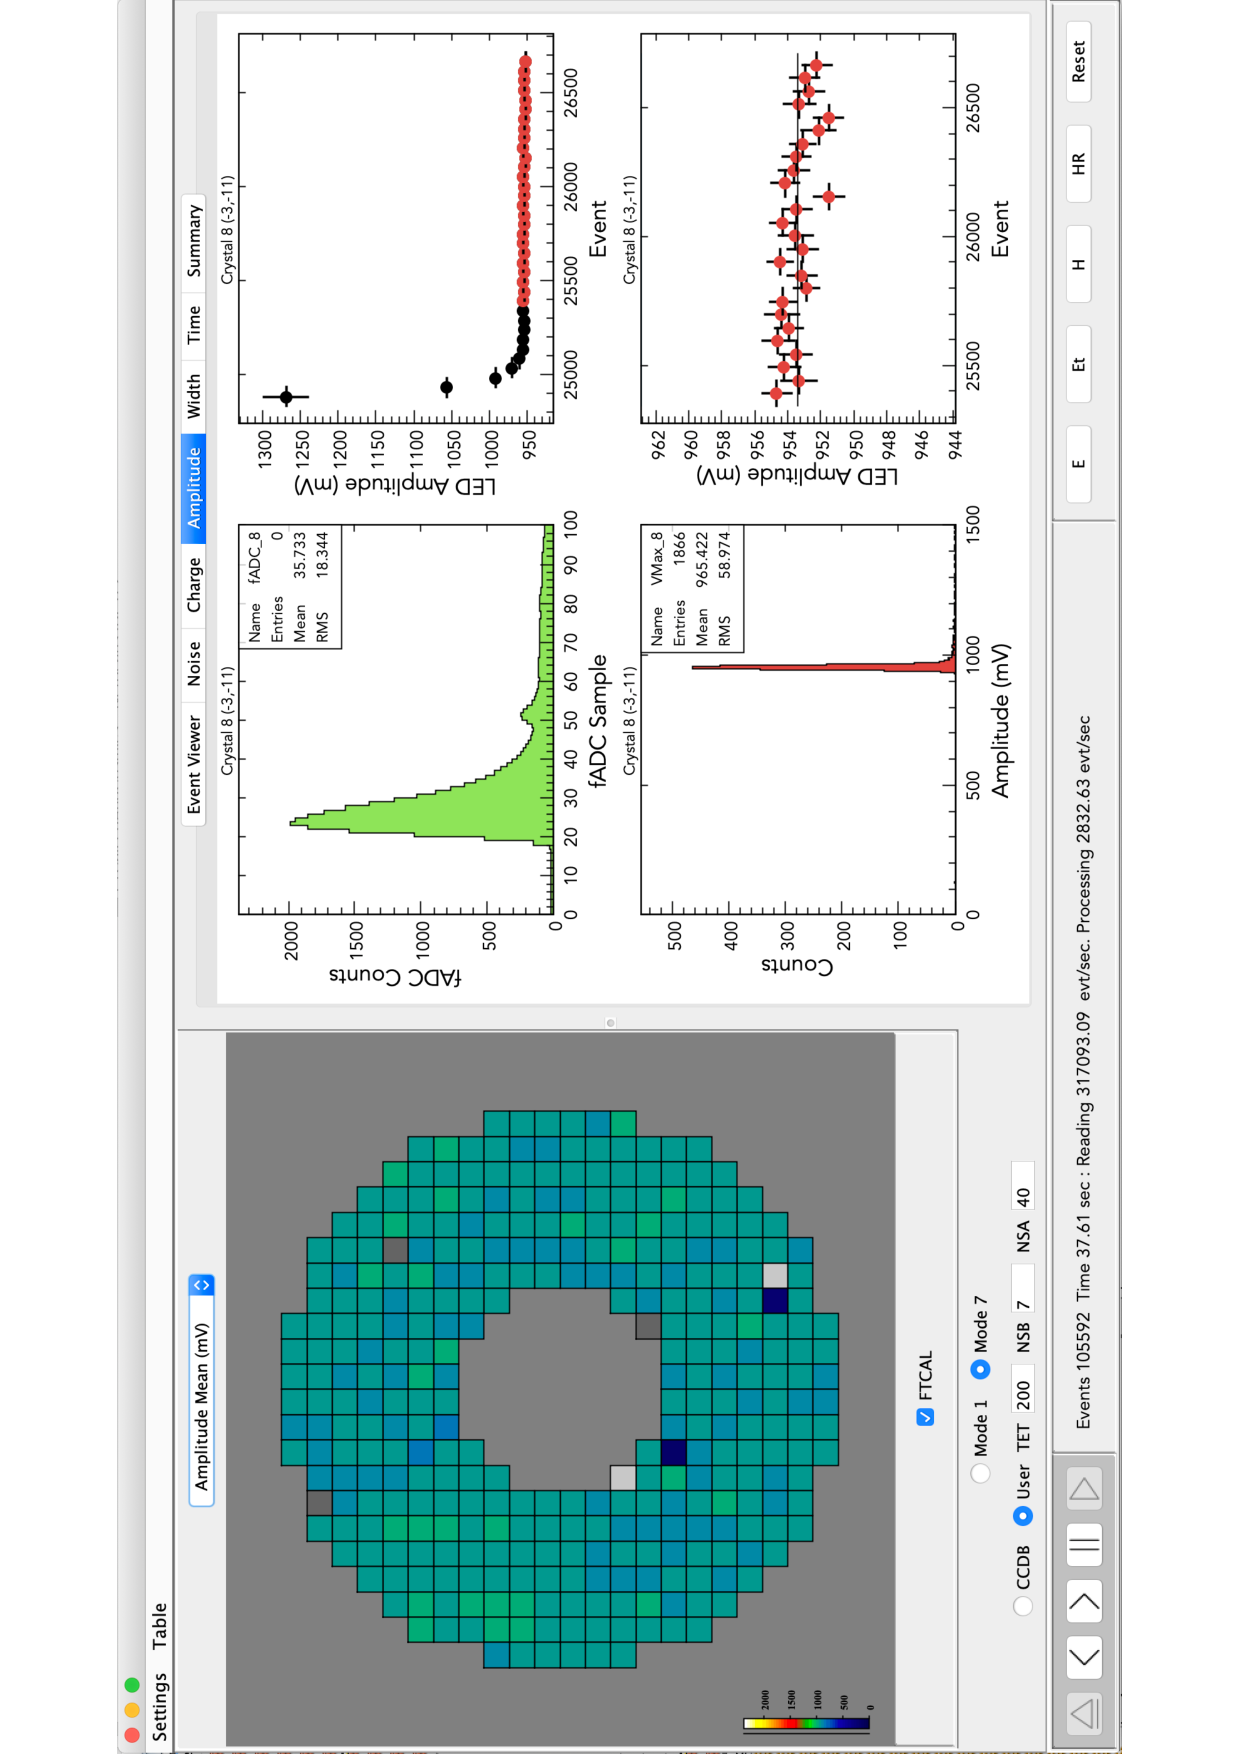
\includegraphics[height=1.0\columnwidth,angle=270]{fig/ftcal_ledrun.pdf}
\caption{Results of a typical FTCal LED run. The left part of the calibration suite display shows a view of the calorimeter with a color scheme representing the LED pulse amplitude. The right part of the panel shows for the selected crystal the average pulse shape (top left), the pulse amplitude as a function of the event number, i.e. of time (top right), the distribution of the amplitudes (bottom left) and the pulse amplitude  as a function event number after the LED has reached stability (bottom right). The latter is fitted to a constant to determine the pulse amplitude that us displayed in the detector view.}
\label{fig:ftcal_ledrun}
\end{figure}

The final mean of calibration without beam is based on the study of the detector response to cosmic rays. A special FPGA-based trigger was developed by the JLAB Fast Electronic Group to select events where a cosmic ray crosses the calorimeter primarily in the vertical direction, i.e. crossing the crystals along the short side. This is achieved by requesting to have a minimum number of signals above threshold in the crystals that are in a "column" of the calorimeter assembly. This is achieved by exploiting the functionalities of the JLAB fADCs and VTPs \cite{daq,trigger}. For these events, waveforms for all crystals in the calorimeter are recorded and analyzed offline using the FT-Cal calibration suite. Details of the analysis procedure are reported in Refs.~\cite{cosmics1,cosmics2}; here we summarize only the main steps and results. For each crystal, events where at least $N_{min}$ crystals with signal above thresholds are found in a vertical range of $N_{range}$ crystals above or below the chosen one. After optimization, the values of $N_{min}$ and $N_{range}$ were fixed to 4 and 5, respectively. For these events, the crystal waveform is integrated in a fixed range and pedestal subtracted to extract the charge. The integration range was optimized empirically to maximize the signal to noise ration compatibly with the signal time jitter  with respect to the trigger. The charge distribution for all selected events in the given crystal is then fitted with a Landau summed to an exponential function, representing the minimum ionizing particle deposition and noise, respectively. The mean of the Landau function, compared to the expected average energy deposition estimated to be 15.3 MeV via GEANT4 simulations, is then used to evaluate the charge-to-energy conversion factor for each crystal. 
\begin{figure}
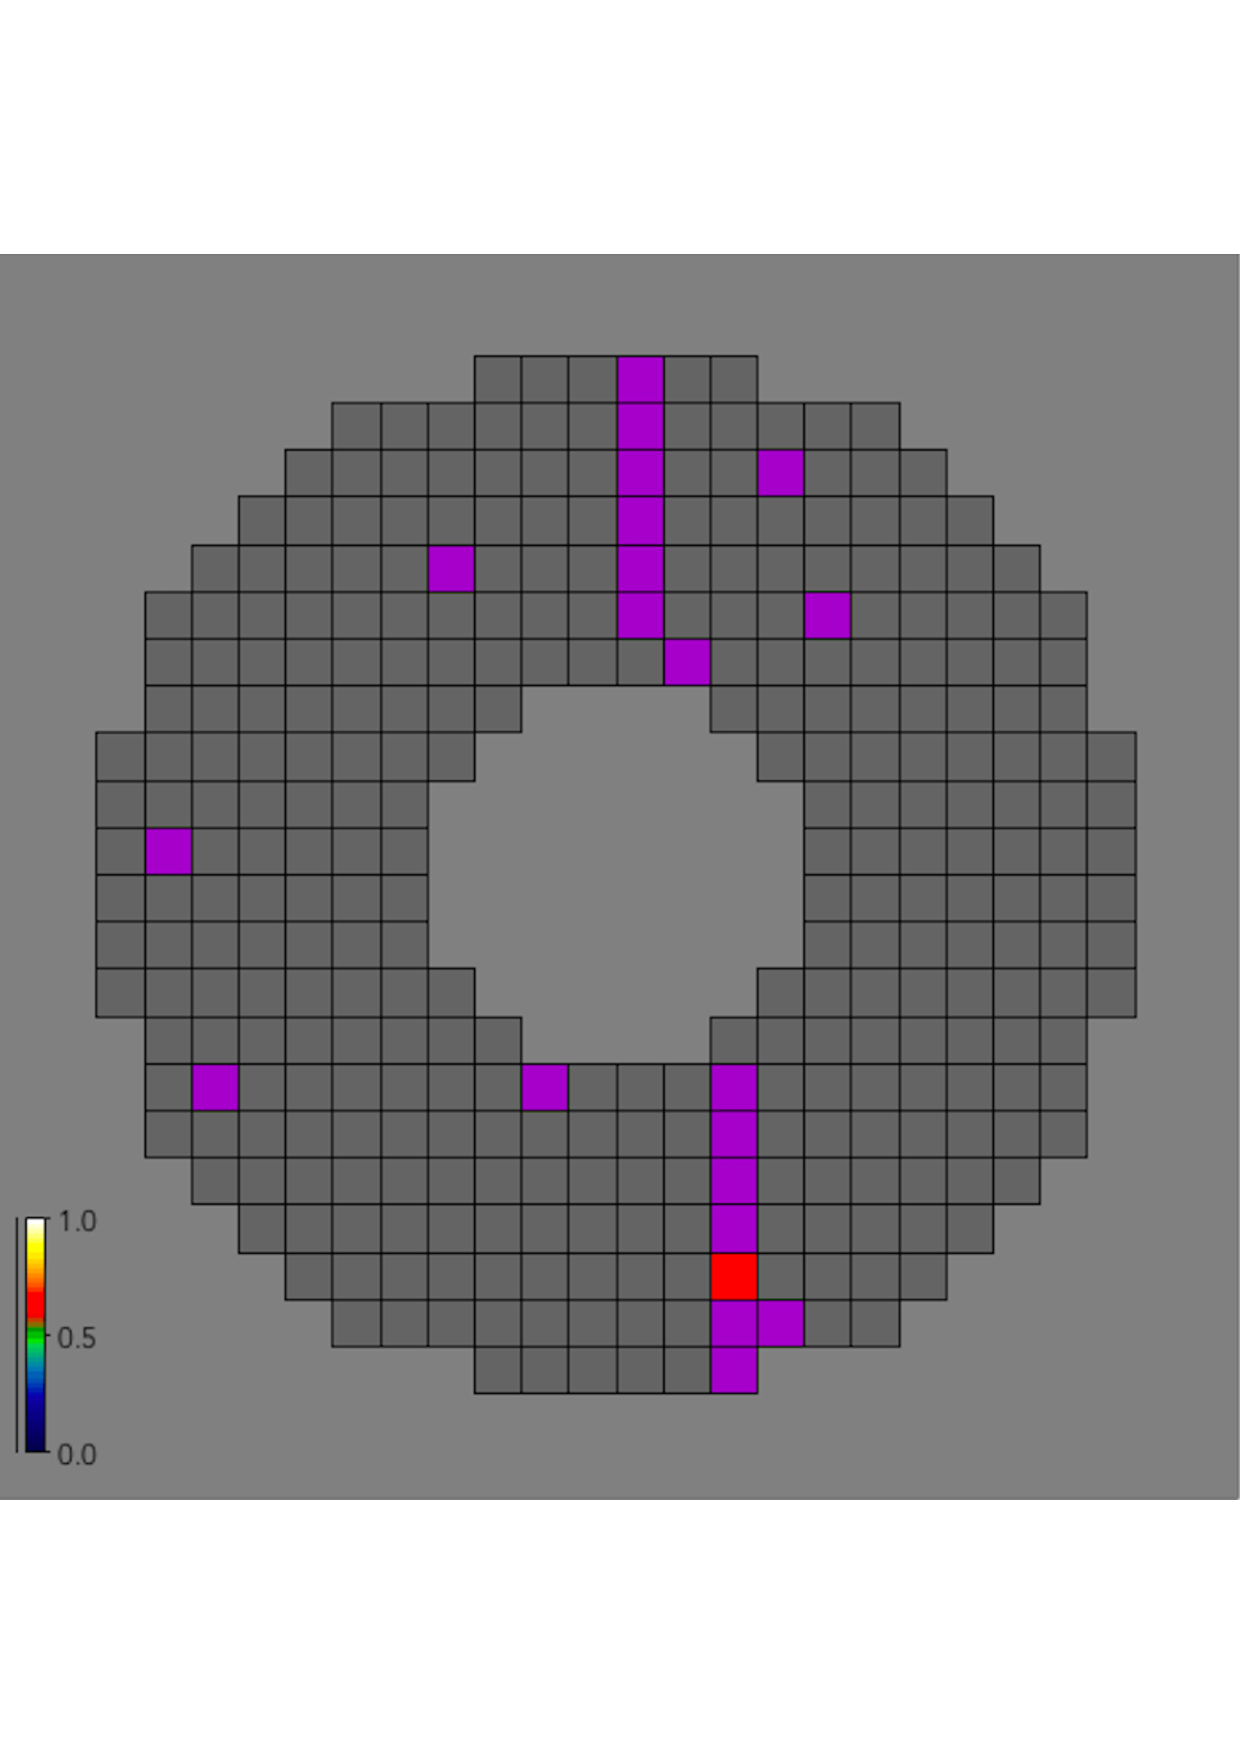
\includegraphics[height=0.58\columnwidth]{fig/ftcal_cosmicview.pdf}
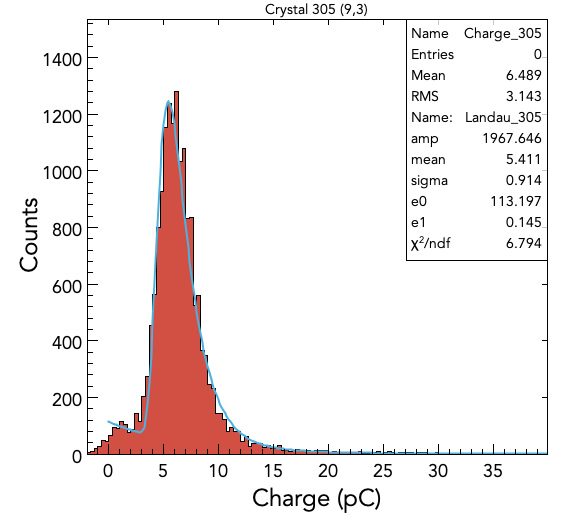
\includegraphics[height=0.5\columnwidth]{fig/ftcal_cosmiccharge.png}
\caption{Left: example of a cosmic ray crossing the calorimeter vertically as displayed by the calibrations suite. Right: example of the measured charge distribution measured from the selected events for a calorimeter crystal; the blue line shows the results of the Landau plus exponential fit; the mean of the Landau function is used to estimate the charge-to-energy conversion factors.}
\label{fig:ftcal_cosmic}
\end{figure}
Fig. \ref{fig:ftcal_cosmic} shows an example of a cosmic ray event as displayed by the calibration suite and an example of the charge distribution for a selected crystal obtained by integrating over the selected events. The typical values of the Landau means are found to be in the range of 4-7 pC at the calorimeter operating temperature of $0^\circ$ C and the corresponding conversion factors in the range of 2.2-3.8 MeV/pC. These values were used as calibration constants for the initial reconstruction of beam data, finding that these usually lead to overestimate by 20\% the actual energy deposited in the energy range of interest for the calorimeter, i.e. 0.5-4.5 GeV. While this discrepancy is significant, it is not unexpected given the uncertainties in extracting the cosmic ray signal from the noise and the two order of magnitudes between the cosmic ray calibration point and the energy range for beam induced signals.

\subsubsection{FT-Hodo pre-beam calibration}
Similarly to the calorimeter, initial checkout of the hodoscope is performed via pulser runs to check the functionality of each electronic channel and evaluate the SIPM gains by measure the Single Photo-Electron (SPE) signal. An external clock is used to trigger the data acquisition recording the waveform of all the 232 channels in a 400 nS windows. The waveforms can be analyzed online by connecting the calibration suite to the DAQ ET ring or offline reading from file. The parameters that are monitored are the pedestal values, the pedestal RMS and the electronic noise. The extracted values are compared to the typical ones to identify problematic channels and disconnected cables. For each channel, waveforms that exceed a minimum threshold above the baselines are analyzed to extract the SPE signal. For this purpose, the waveforms are integrated in a fixed time range and pedestal subtracted. The distribution of the extracted charge for a selected channel is shown in Fig. \ref{fig:fthodo_spe}. Clear peaks corresponding to one, two and three photo-electrons are visible; the difference between two peaks is used to determine the gain of the channel finding typical values of the order of 20~pC.
\begin{figure}
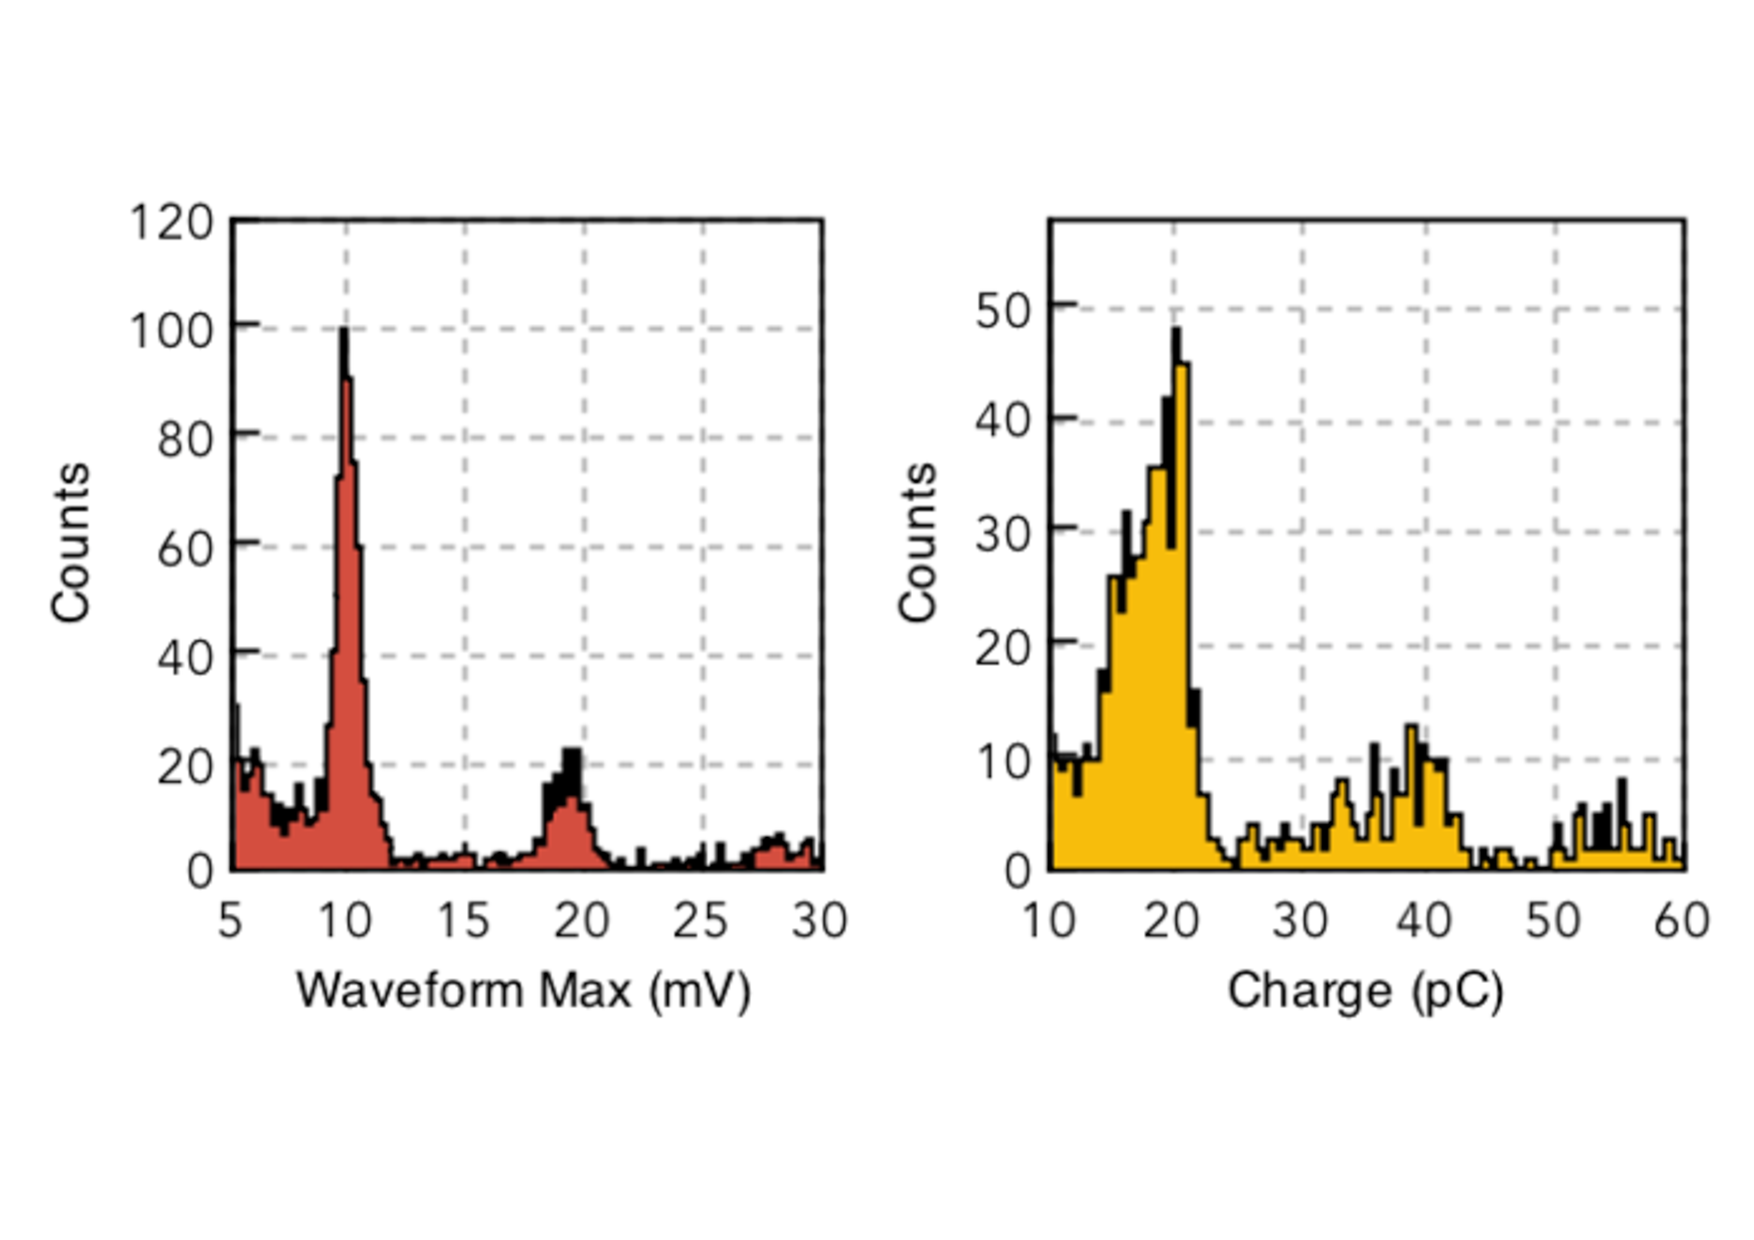
\includegraphics[width=1.0\columnwidth]{fig/fthodo_spe.pdf}
\caption{SPE signal from a single Hodoscope SiPM in mV (left) and pC (right) determined using the waveform max and integral respectively.   }
\label{fig:fthodo_spe}
\end{figure}

Further checkout of the detector is performed via cosmic ray data taking. The same FPGA based trigger developed for the calorimeter is used to trigger the DAQ on events in which multiple tiles of the hodoscope have a signal above threshold. For such events, all hodoscope channel waveforms are recorded and analyzed offline. The signal charge is extracted integrating the waveform in a fixed time window and subtracting the pedestals. The resulting charge distributions are inspected to ensure a sizable signal for all tiles. In this case no attempt is made to extract the charge-to-energy conversion factor from these distributions because of the unfavorable orientation of the hodoscope in the installation position for the measurement of cosmic ray that can cross the scintillation tiles with a very large angular spread and therefore of path lengths within the active volumes.

\subsubsection{FT-Trk pre-beam calibration}
The initial checkout of the FT tracker and in particular of the front-end electronics is performed by means of pedestal and pulser runs. Since these procedures are standard for the CLAS12 MicroMegas detectors, we refer to Ref. \cite{mm} for further details.

\subsection{On-beam calibration and commissioning}
While pre-beam calibration are essential to ensure all detector components are fully operational, the final calibrations to extract the parameters needed for the FT reconstruction are based on analysis of beam data. Here we report specifically on the procedures developed for the calibration of the calorimeter and hodoscope, since no specific calibrations are needed for the tracker.

For both hodoscope and calorimeter, energy and time calibrations can be obtained from the analysis of data recorded with the CLAS12 production triggers and do not require dedicated data taking. A dedicated run is typically employed, however, for matching the gains from all Hodoscope SiPMs~\footnote{Having a matched gain from all Hodoscope SiPMs allows having a common VTP threshold for all channels. }. In this dedicated run, average MIP signals are obtained for a set of different HV settings (see Fig.~\ref{fig:fthodo_gainmatch.pdf}), determining two constants from which gain matching is established.
\begin{figure}
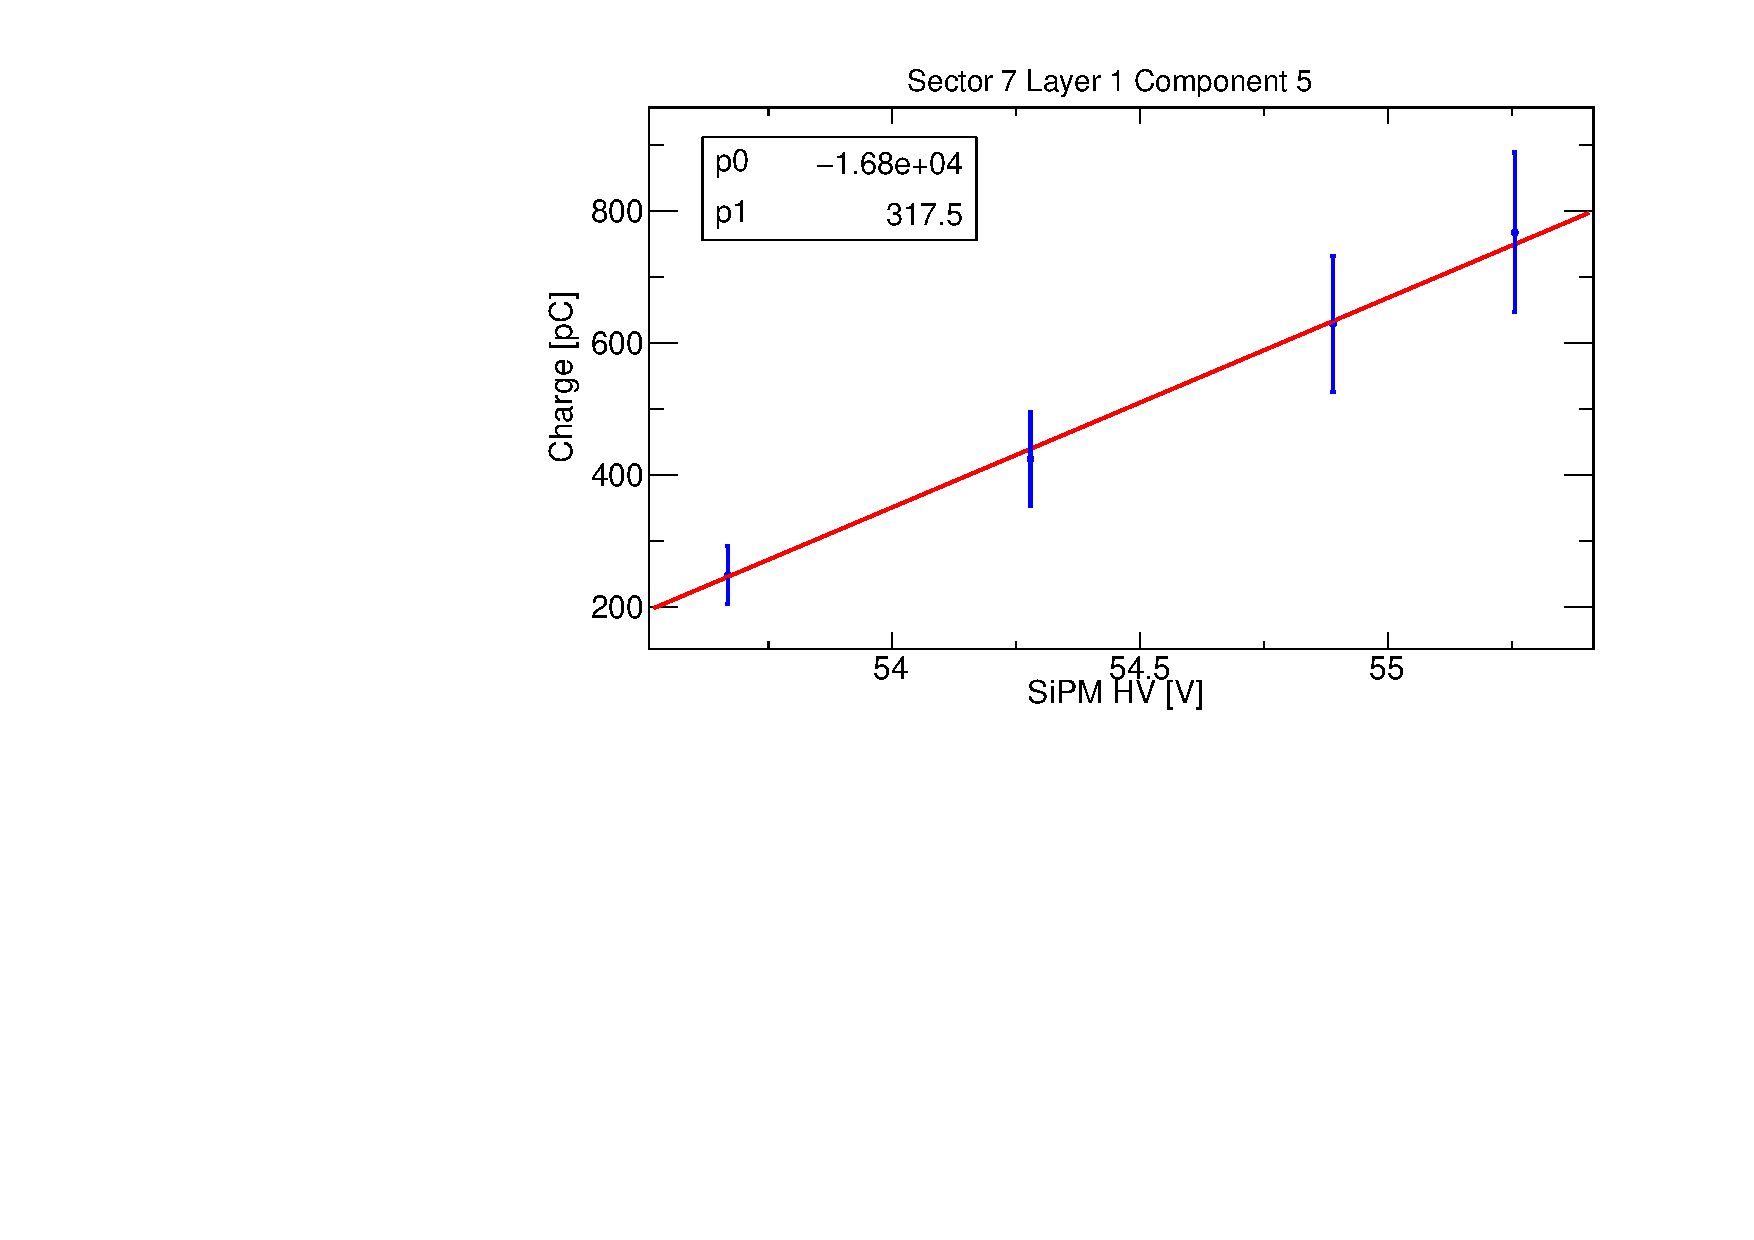
\includegraphics[width=1.0\columnwidth]{fig/fthodo_gainmatch.pdf}
\caption{Gain-matching constant determination for a single SiPM.}
\label{fig:fthodo_gainmatch}
\end{figure}


Energy calibration for the FT-Cal is achieved by analyzing electron elastic scattering events or by reconstructing the $\pi^0\to\gamma\gamma$ decay where both photons are detected in the calorimeter. 

\begin{figure}

\includegraphics[height=1.0\columnwidth]{fig/dummy.png}
\caption{aaa}
\label{fig:ftcal_elasticcal}
\end{figure}
Elastic scattering calibration was found to be particularly effective at low beam energy and was performed using 2.2 GeV beam data recorded during the CLAS12 engineering run. Events with only one cluster in the FT-Cal were selected and, based on the existing cosmic ray calibrations, the energy of the crystal with the largest signal, i.e. the {\it seed}, was extracted. For crystal, these events were accumulated requesting the seed energy to be larger than 55\% of the total cluster energy. The right edge of the distribution of the seed energy was fitted with a Gaussian function to extract the peak position. The mean value of the Gaussian function was compared to what expected based on GEANT4 simulations to extract a correction to the charge-to-energy conversion factor used in the cluster reconstruction. Fig.~\ref{fig:ftcal_elasticcal} shows an example of the seed energy distribution and the cluster energy distribution for a selected crystal. Using these constants, an energy resolution of  3.3\% at 2.2 GeV beam energy was determined by fitting the reconstructed elastic peak (see Fig.~\ref{fig:ftcal_elasticres}). With the same calibration constants, the $\pi^0\to\gamma\gamma$ decay was reconstructed at 10.6 GeV beam energy selecting events with both photons detected in the FT-Cal, finding the width of the $\pi^0$ peak is of the order of $\sim 4.4$ MeV.
\begin{figure}
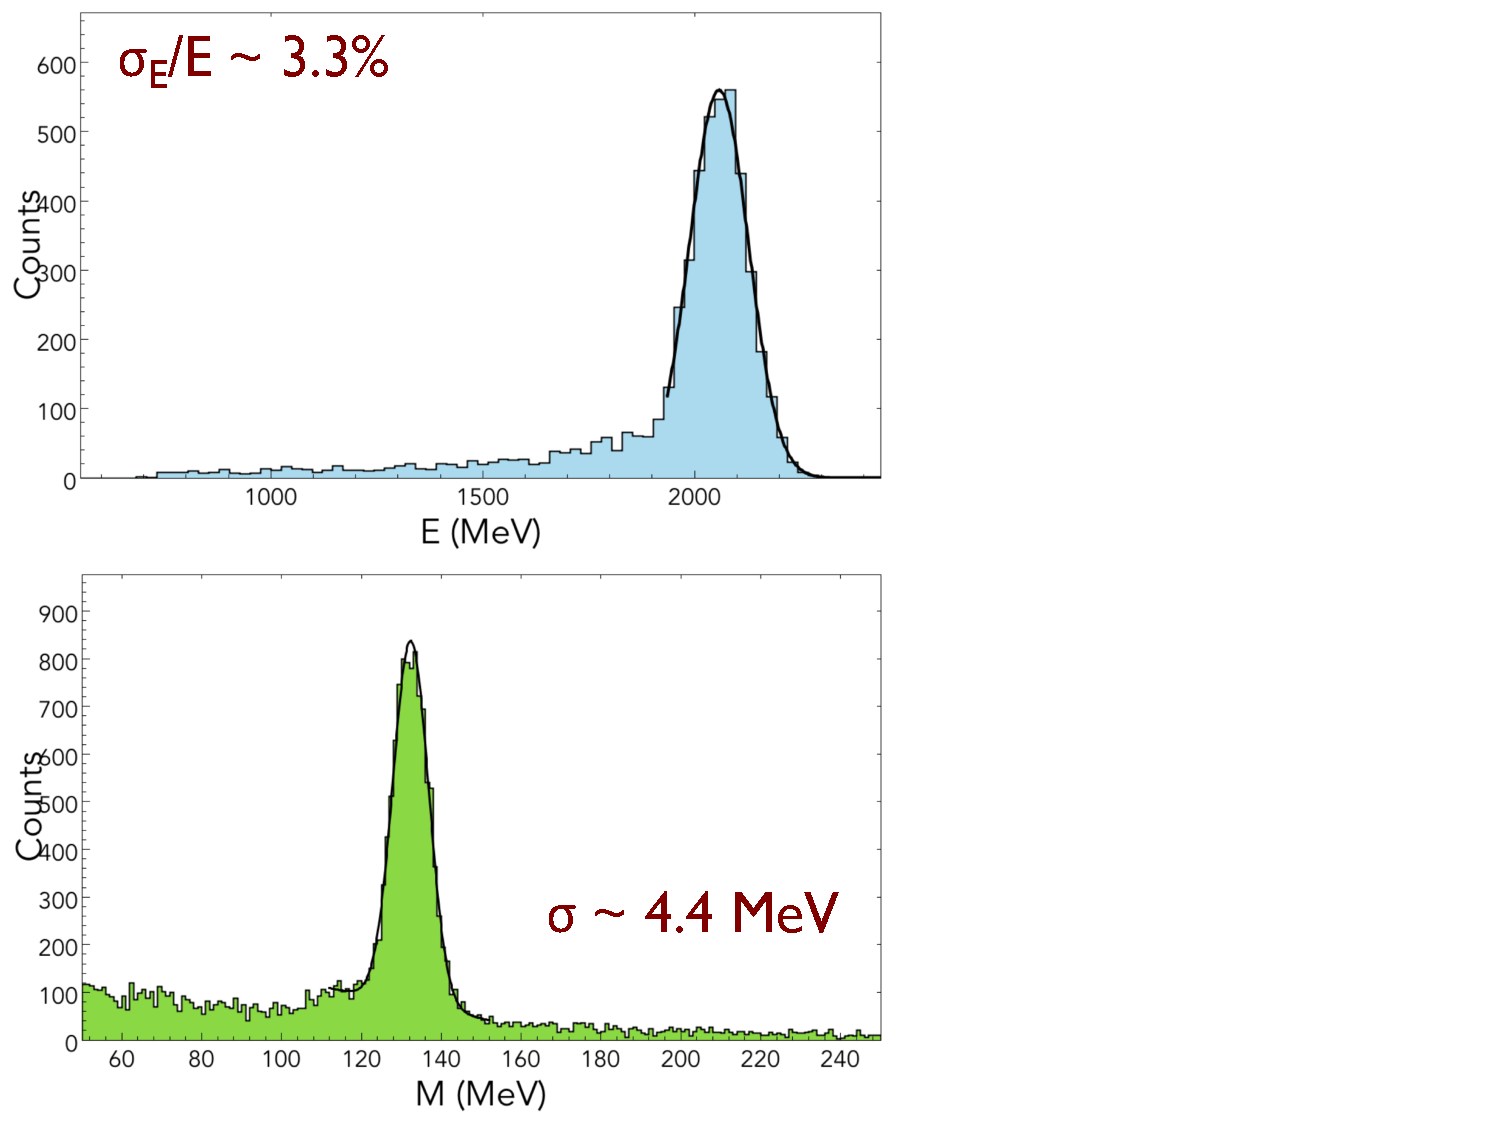
\includegraphics[height=1.0\columnwidth]{fig/ftcal_elasticres.pdf}
\caption{Left: electron energy spectrum reconstructed at 2.2 GeV beam energy in the FT-Cal; the peak corresponds to elastic scattering; after calibrations based on elastic events, an overall energy resolution of 3.3\% at 2.2 GeV is found. Right: $\pi^0\to\gamma\gamma$ invariant mass spectrum reconstructed at 10.6 GeV beam energy using the elastic scattering energy calibrations: the width of the $\pi^0$ peak determined via a Gaussian fit was found to be of $\sim 4.4$ MeV.}
\label{fig:ftcal_elasticres}
\end{figure}

Since the effectiveness of the elastic calibration is limited to beam energy of the order of few GeV because of rapid decrease of the corresponding cross section at higher energies, an alternative approach was develop to perform the energy calibration of the FT-Cal based on the the $\pi^0\to\gamma\gamma$ decay. Events where both photons are detected in the calorimeter were selected and filtered applying the following cuts:
\begin{itemize}
    \item the energy of both clusters, as reconstructed based on existing calibrations is larger than 500 MeV,
    \item the size of both clusters, i.e. the number of crystals involved, is larger than 3,
    \item the opening angle between the two clusters is larger than $2^\circ$ deg.
\end{itemize}
The last cuts is useful to reduce background resulting from split clusters.  For each crystal, events in which the crystal is the seed of one of the two clusters are accumulated and the ratio between the measured cluster energy for the given crystal and the energy calculated from the nominal $\pi^0$ mass and the other cluster energy is computed. The distribution of such ratios is fitted with a Gaussian function to derive a correction factor for the charge-to-energy calibration constant of the selected crystal. The procedure is applied iteratively until the $\pi^0$ mass spectrum for all crystal is within 0.5 MeV from the nominal value. Fig.~\ref{fig:ftcal_pi0} shows an example of the ratio distribution and of the $\pi^0$ mass spectrum for a selected crystal before and after (blue histogram) the calibration procedure. The advantage of this procedure is that it does not strongly depends on the beam energy and exploits the full energy spectrum of the clusters providing a check of the linearity. The left panel of Fig.~\ref{fig:ftcal_pi0} shows the  correlation between the measured and computed cluster energies after calibrations: the energy range, which is covered with good statistics, is from 0.5 to 5 GeV with a perfect overlap with the energy range of interest for the FT. The resolution that is achieved with this calibration algorithm is of the order of 4-5 MeV integrated  on the whole calorimeter as  shown by the right panel of Fig.~\ref{fig:ftcal_pi0res}.

\begin{figure}
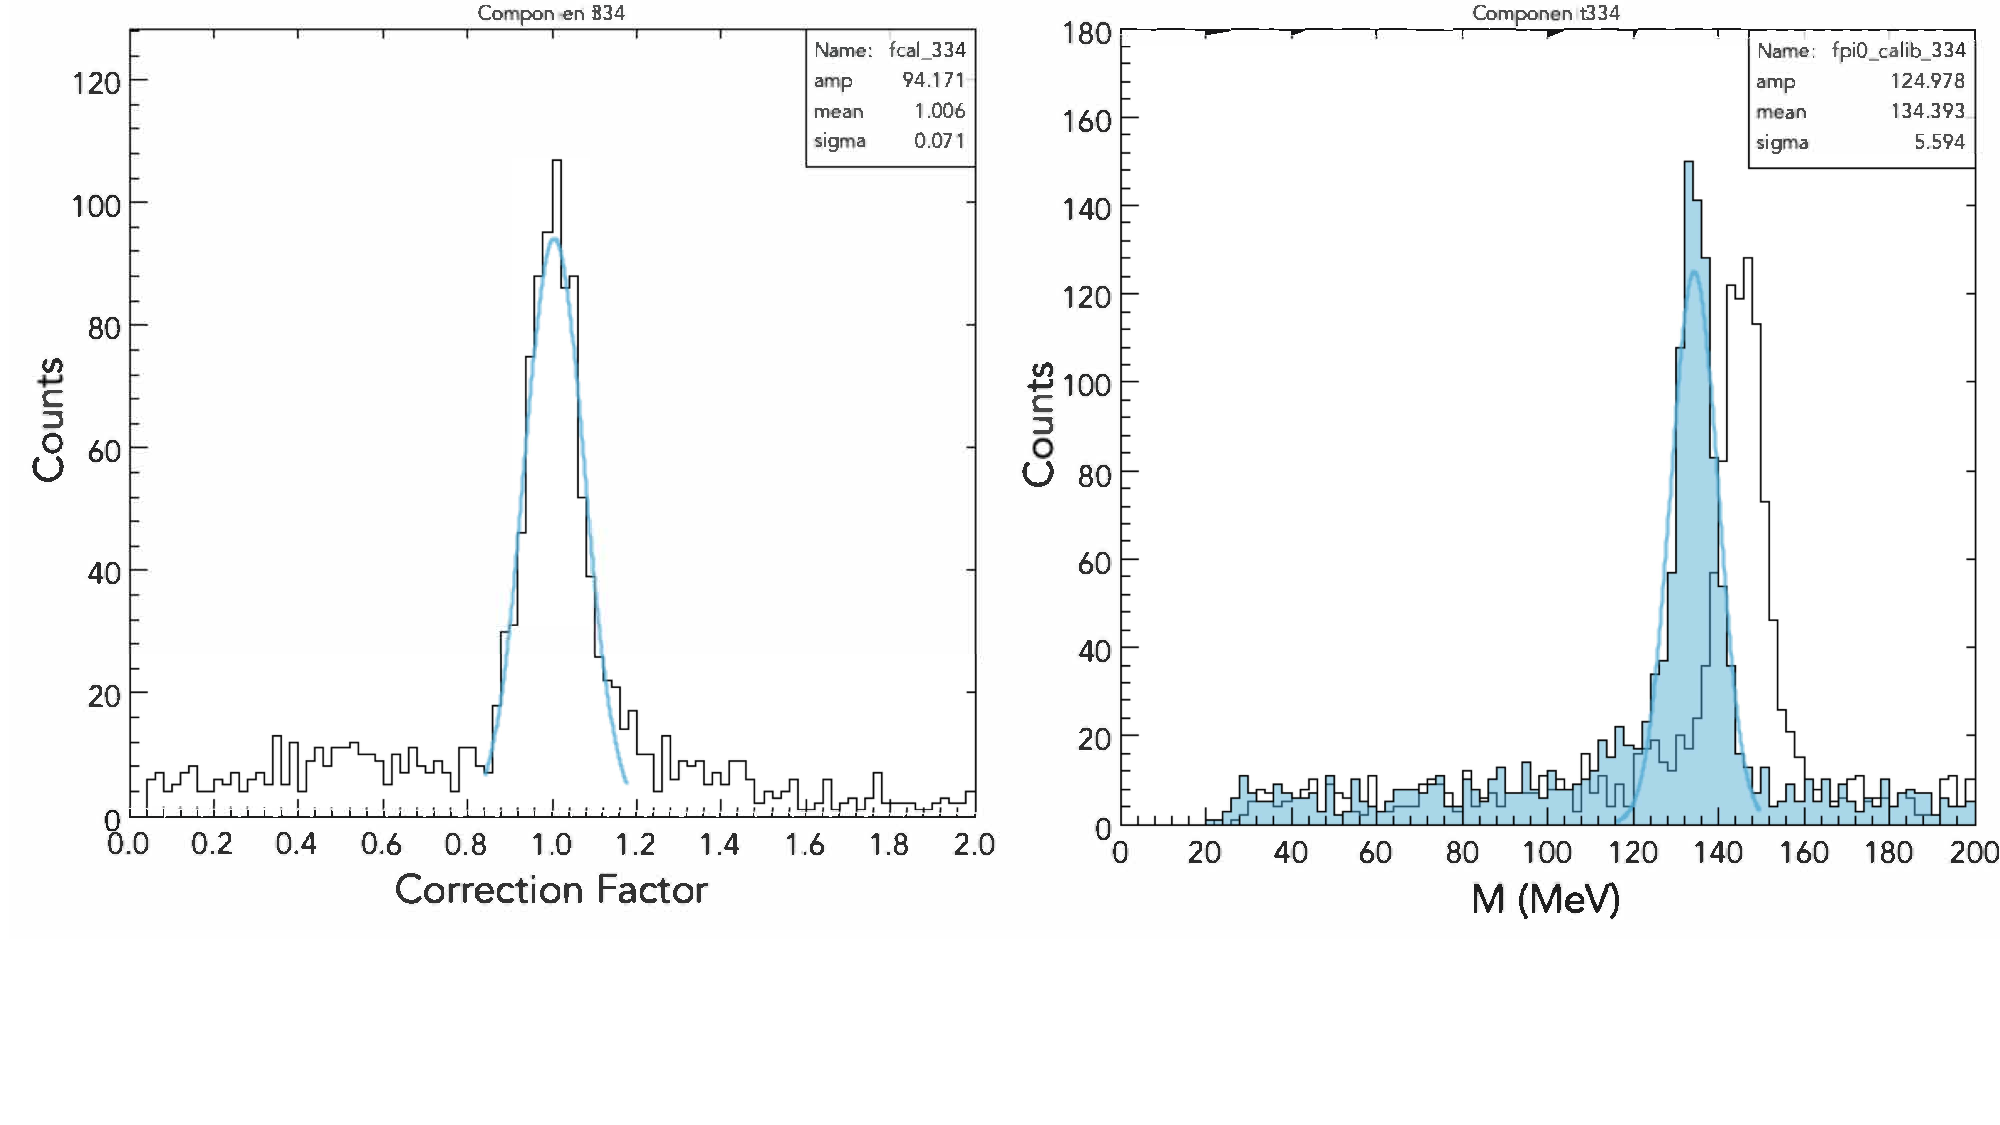
\includegraphics[height=0.46\columnwidth]{fig/ftcal_pi0.pdf}
\caption{Left: calibration correction factor for a selected crystal computed as the ration between the measured energy of clusters where the crystal is the seed and the energy calculated from the nominal $pi^0$ mass and the other cluster energy. Right: $\pi^0$ mass spectrum for the same crystal before and after the calibration procedure.}
\label{fig:ftcal_pi0}
\end{figure}

\begin{figure}
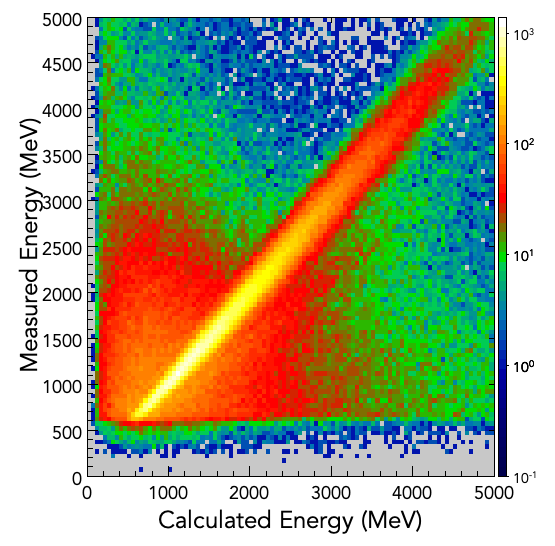
\includegraphics[height=0.48\columnwidth]{fig/ftcal_pi0linearity.png}
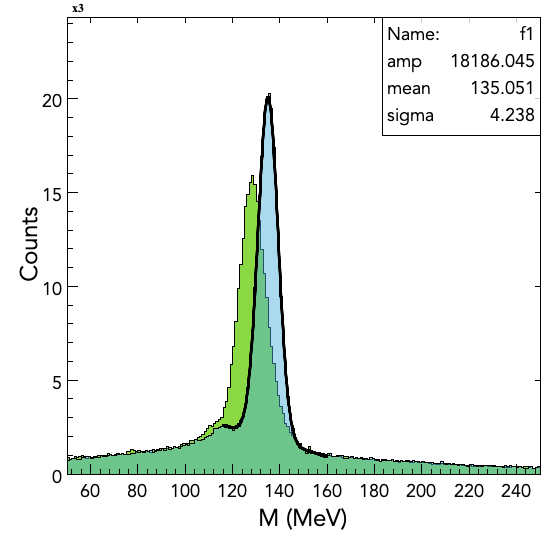
\includegraphics[height=0.48\columnwidth]{fig/ftcal_pi0resolution.png}
\caption{Left: correlation between the measured cluster energy and the energy computed from the nominal $\pi^0$ mass; the range covered is well match to the FT energy range of interest. Right: $\pi^0$ mass spectrum before (green) and after (blue) the calibration; the achieved resolution id of $\sim 4.2$ MeV.}
\label{fig:ftcal_pi0res}
\end{figure}

Energy calibration of the FT-Hodo is performed by studying the energy deposition of minimum ionizing particles. Fig.~\ref{fig:fthodo_mips} shows the charge from MIP signals in the thin and thick tiles. For the FT-Hodo, charge particle signals are selected by requiring the geometrical matching of tiles in the two layers. The distribution are fitted with a Landau plus an exponential function to determine the average MIP charge. The charge-to-energy conversion factors are determined by comparing the resulting values to the ones estimated from GEANT4 simulations.
\begin{figure}
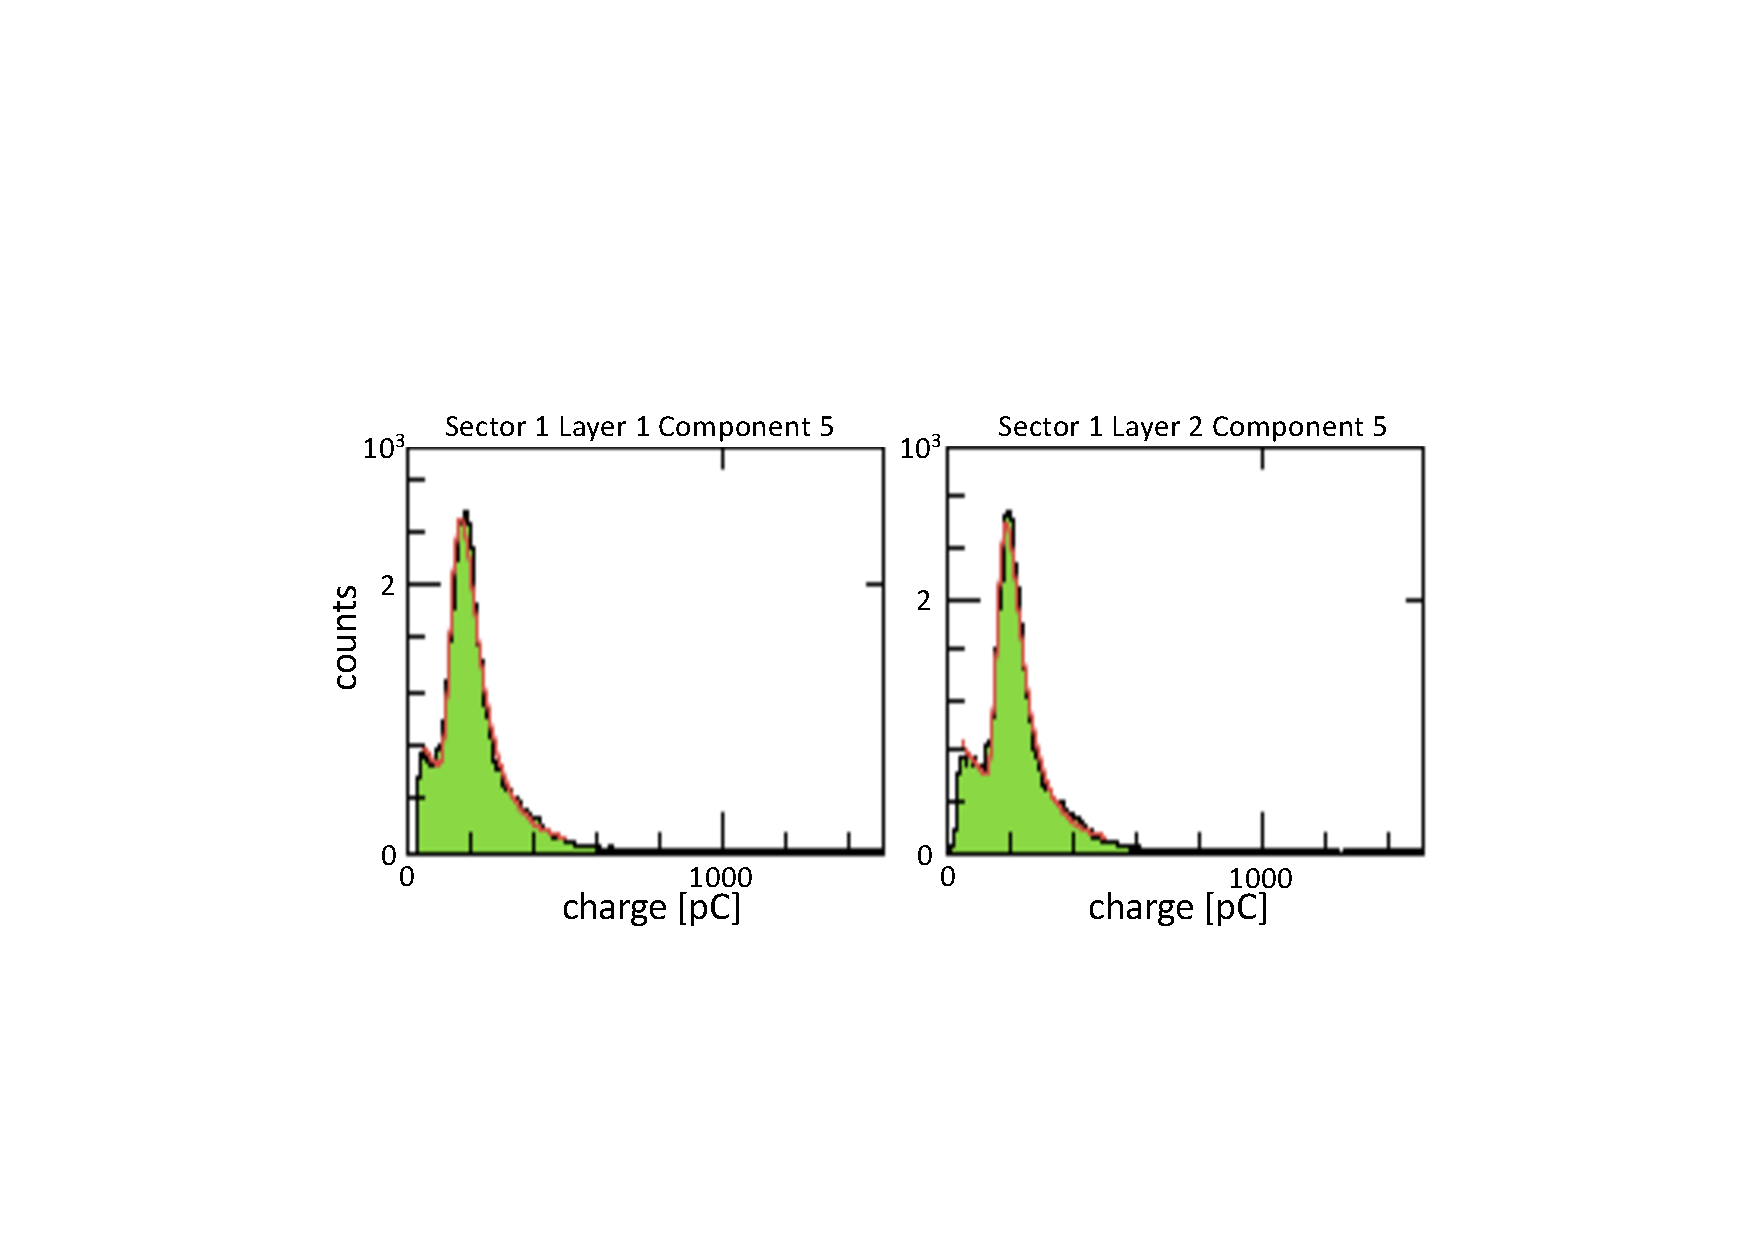
\includegraphics[width=1.0\columnwidth]{fig/fthodo_mips.pdf}
\caption{Signal from two Hodoscope tiles (thin and thick layer) fitted with a Landau plus an exponential to established the charge-to-energy constants.}
\label{fig:fthodo_mips}
\end{figure}

Timing calibrations of both the FT-Cal and FT-Hodo are obtained by studying the time correlation of the signals detected in the two detectors and the CLAS12 Forward Time-Flight (FTOF) detector~\cite{ftof}. Events with a scattered electron in the CLAS12 forward detectors and a second particle is detected in the FT are selected. In such events, the start time $t_0$, i.e. the time of interaction of the beam electron in the target, can be computed from the electron FTOF time subtracted of the time-of-flight from the vertex to the FTOF. The start time can then be used as a reference for the calibration of the FT detectors. 

For the FT-Hodo, the signal time, $t_{hit}$, subtracted of the time-of-flight from the vertex to the detector, is compared to the event start time, $t_0$. The difference between the two gives the time correction needed. Fig.~\ref{fig:fthodo_time} shows an example of the time offset distribution for a thin and a thick tile.
\begin{figure}
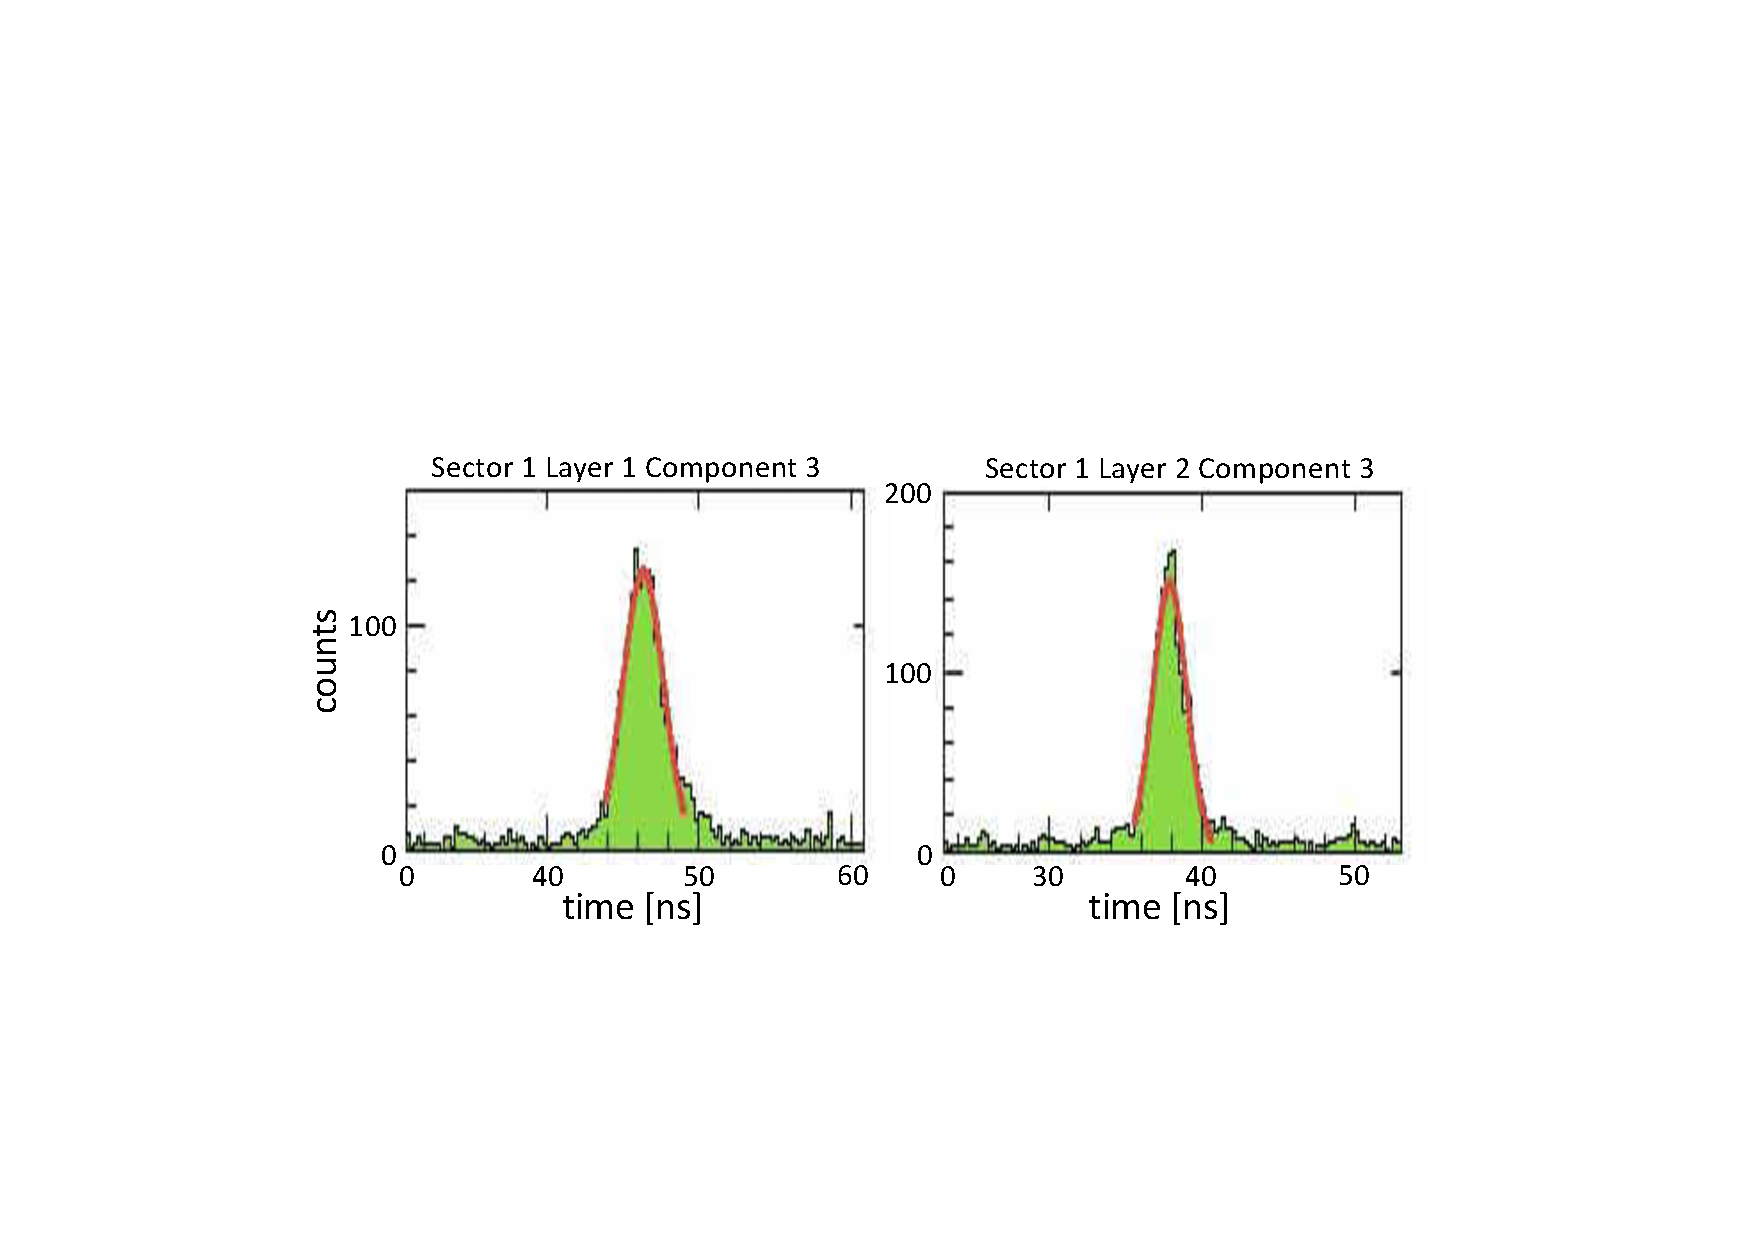
\includegraphics[width=1.0\columnwidth]{fig/fthodo_time.pdf}
\caption{FT-Hodo time correction determined by Gaussian fits on the time difference between the time-of-flight substracted signal time and event start time.}
\label{fig:fthodo_time}
\end{figure}

The same procedure is used for the FT-Cal, for which however all hits with energy greater than 10 MeV are used with no requirements on the charge of the associated particle. The use of such low energy threshold is important to be able to calibrate the crystals that are on the edges of the calorimeter. The measured time is then compared with the event start time, extracting both an overall offset and a charge-dependent correction, associated. to a time-walk effect. The top-left panel of. figure Fig.~\ref{fig:ftcal_time} shows the time offset as  a function the signal charge; this histogram profile is fitted to a power low, $a/q^\lambda$, as shown in the top-right panel to determine the time-walk correction. After applying this correction, the time offset distribution shown in the bottom plots  of the same figure are fitted to a simple Gaussian function to determine the global offset. The bottom right is the  final distribution with all corrections, showing a clear  coincidence peak at 0 surrounded by the accidental peaks at multiple of $\pm  4.008$ ns  due to the RF beam structure. The time offset constant term is extracted for each crystal separately, while the time walk constants are fitted for all crystal together since no significant difference between crystals was found. 

\begin{figure}
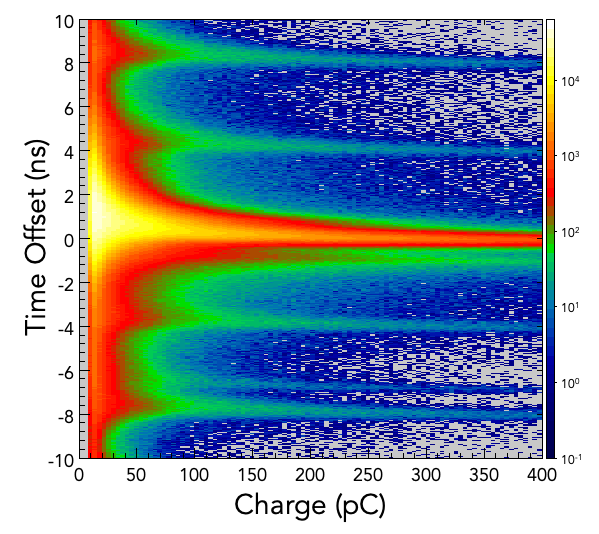
\includegraphics[height=0.42\columnwidth]{fig/ftcal_twbefore.png}
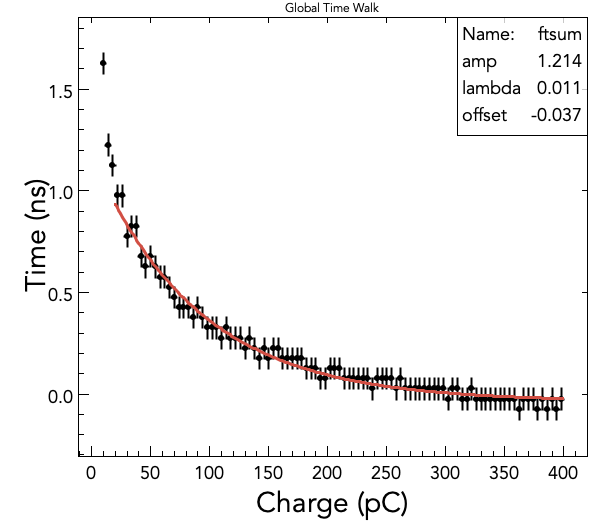
\includegraphics[height=0.42\columnwidth]{fig/ftcal_twfit.png}
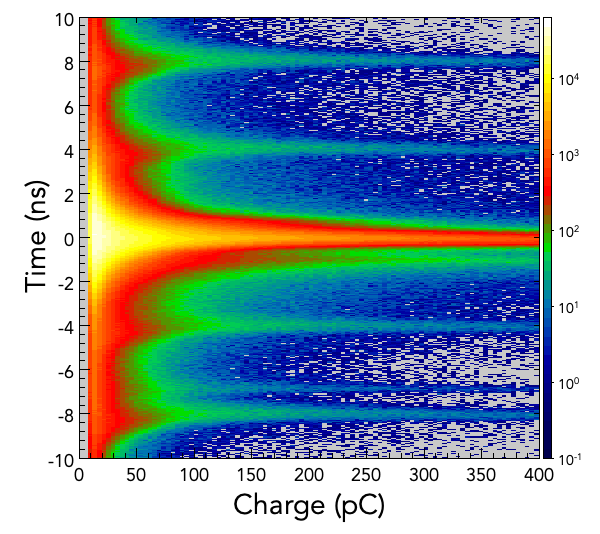
\includegraphics[height=0.42\columnwidth]{fig/ftcal_twafter.png}
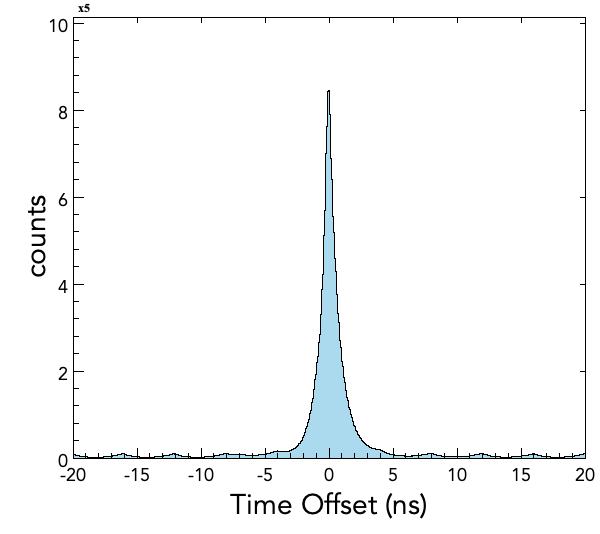
\includegraphics[height=0.42\columnwidth]{fig/ftcal_timefinal.png}
\caption{Top: FT-Cal time offset dependence on the charge (left); the profile of the histogram is fitted to a power law, $a/q^\lambda$. Bottom: FT-Cal time offsets after the time walk and the subtraction of the residual constant term.}
\label{fig:ftcal_time}
\end{figure}

